\section{Literature Review}
\setlength{\parindent}{10ex}
In this review, different approaches for predicting bathymetry are discussed.
The two main methods for collecting bathymetry data are \ac{SDB} and \ac{EGM}.
There is also a third approach discussed that improves upon the idea of an \ac{EGM}.
\ac{MBES} for precise measurements of bathymetry \cite{farr1980multibeam} is also covered.
The \ac{ML} models used for training are explained in detail as well.

\subsection{Machine Learning}
Machine Learning can be defined as the process of fitting a model to data with an algorithm \cite{bishop2006pattern}.
Predictions can then be produced from the models by inputting new data.
To validate the predictions, the supplied data's result is known.
For example, when a model is trained to predict if an image contains a car, data from the images is extracted and used to train the model.
Images with cars are considered positive images.
Images without cars are considered negative images.
New images that are labeled as positive or negative are given to the model for validation.
If the model successfully predicts the labels, it will have a high accuracy and be a "valid" model.

\par
The two main types of models in Machine Learning are classification and regression.
There are several high-level descriptions of classification and regression models including supervised learning, unsupervised learning, and reinforcement learning.

\par
Classification models that predict a discrete value, for example whether an image contains a car.
The model predicts a discrete value of either positive or negative.
These types of models are effective at predicting values that can be grouped into "labeled" data.
Data is labeled when it is assigned an output value as a "truth" label.
For example, to train a model to detect cars, the model must be supplied with labeled images. 
The labels are either positive (there is a car in the image) or negative (there is not a car in the image).
This labeling describes a "binary" classification, meaning there are two options from which to choose.
Classification models can also be combined to form ensemble models.
An ensemble is a combination of weaker predictors to form a strong predictor.
%Include citations BELOW!!!!!
Examples of classification models used in this project include: Decision Trees, Naive Bayes, MLP Classifier, Quadratic Discriminant Analysis Classifier, and K Nearest Neighbors Classifier.
Examples of ensemble classifiers used in this project include: Random Forest Classifier, Ada boost, Gradient Boosting, Bagging, and Voting.

\par
Regression models predict a continuous value.
For example, predicting the value of a home.
Essentially, this model represents a mathematical function where the input data is the function parameters.
The parameters for the model are predictors for the value of the home.
Predictors for a home include square footage, number of rooms, acrerage, and school distance.
This method is appropriate when the desired result cannot be grouped into discrete "labeled" data.
This is because classification is not ideal for predicting a infinite set of continuous values.

\par
Unsupervised learning describes a model that is trained without labels, that is, the training data does not have corresponding truth values \cite{bishop2006pattern}.
Training a model without "truth" is used for grouping similar values together.
This approach is ideal for identifying correlations in data that is otherwise unrelated and unlabeled.

%Maybe move this above??
\par
Supervised learning describes a model that is trained with labeled truth data. \cite{bishop2006pattern}.
Training is guided or supervised by comparing results to labeled truth data.
This method of training is effective at fitting accurate models, and is used in this project for predicting bathymetry.
All models trained in this project use supervised learning.
Each model used will be discussed in subsequent sections.

\subsubsection{Bias and Variance}
%Describe the Bias and Variance relationship!
The generalized error of a model can be expressed in terms of bias and variance.
Bias is the average error of a model for different training sets, while variance describes the sensitivity of the model to data.
These two terms are necessary to understand the bias-variance problem.
This problem applies to all forms of supervised learning \cite{geman1992neural} and describes the indirect relationship of bias and variance.
Namely that minimizing bias often increases variance, and minimizing variance often increases bias.
Models with high bias will be inaccurate when predicting data not used during training, while models with high variance will overfit \cite{cawley2010over} the training data by modeling noise in the data as opposed to the desired outputs.
Optimally, accurate models should have low bias and variance.

%Include image showing bias and variance here!!
\begin{figure}[htp]
    \centering
    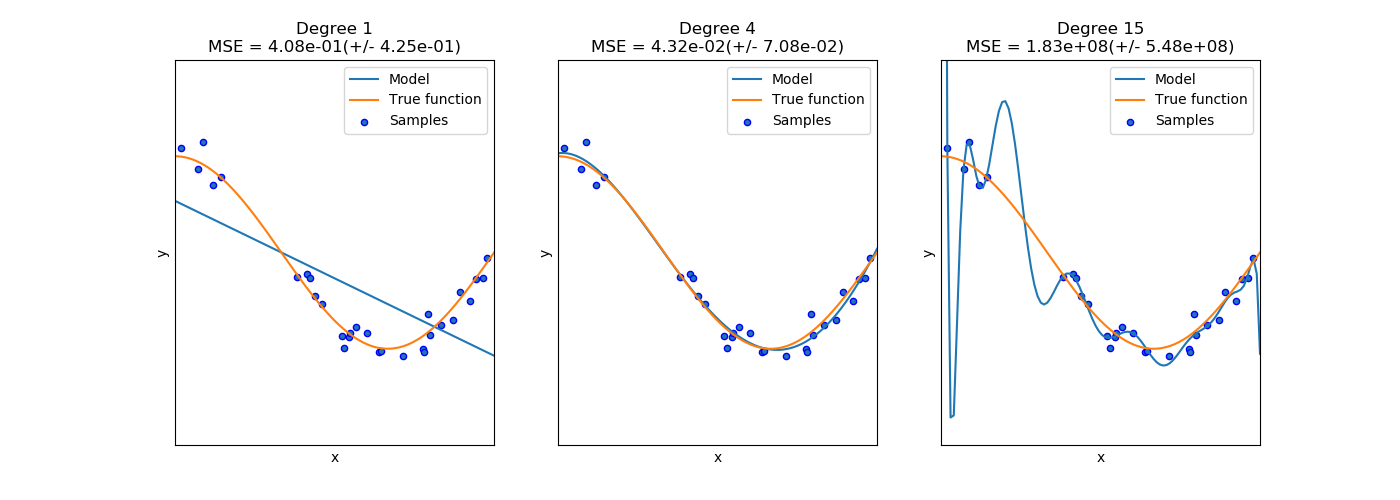
\includegraphics[width=\textwidth]{sphx_glr_plot_underfitting_overfitting_001.png}
    \caption{Three plots of the function \( f(x) = cos(\frac{3}{2} \pi x)\) with noisy samples along the graph. 
    A linear regression model is fit to the samples with orders of 1, 4 and 15.
    The model fit with order 1 does not respond well to changes in the samples and is a great example of high bias.
    The model fit with order 4 fits the function very well and is a example of balanced bias and variance.
    The model fit with order 15 fits the samples too well, but flucuates wildly. 
    It is a excellent example of high variance.}
    \label{}
\end{figure}

\subsubsection{Decision Trees}
%Talk about decision trees here
Decision trees are supervised models used for classification or regression \cite{breiman2017classification}.
However, they are easy to understand and interpret due to their simple decision structure. 
They are susceptible to over-fitting and can create overly complex trees that do not generalize well.
% Maybe put this with Bias and Variance
Over fitting is where a model will fit too closely to a training set \cite{cawley2010over}, making it unable to make accurate predictions on data outside of what was used in training.

\begin{figure}[htp]
    \centering
    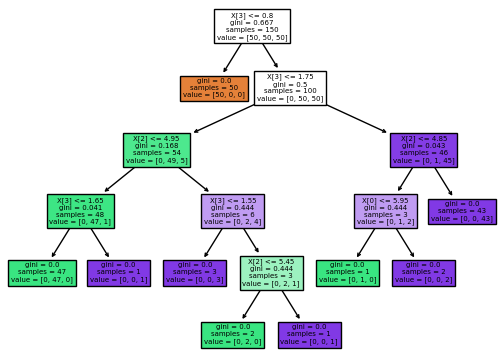
\includegraphics[width=\textwidth]{dtreesepal.png}
    \caption{An example of a decision tree.
    Decision trees work by making binary decisions across a decision boundary.
    Each leaf node represents a classification label and the binary decisions that selected that label.}
    \label{}
\end{figure}

%Talk about random forest here
\par
The Random Forest Classifier is an ensemble of many decision trees \cite{breiman2001random}.
It fits a number of decision trees on various sub samples of the dataset.
This also helps to control over fitting because each tree is fit to a sub sample of the dataset.
It averages the prediction of each tree to make a more accurate prediction than any single tree.


\subsubsection{Boosting}
%Talk about Ada Boost here
Boosting describes a type of ensemble that is concerned with reducing bias.
The idea is to build base estimators sequentially and then use the results of each to train a different estimator with the intention of reducing bias.
Adaboost is an example of one such model \cite{freund1995desicion}.
Its core principle is the fitting of weak learners on many random samples of the training data, which are then combined with a weighted majority vote. 
This process is iterated for the training phase.



%Talk about Gradient Boosting Here
%Need to finish this paragraph....
\par
The gradient boosting classifier is an ensemble of trees similar to a random forest classifier.
In gradient boosting, decision trees are used as "weak" learners.
They are gradually added to the model in order to reduce the error.
This "gradient descent" approach is effective at building a successful classifier.
These types of boosting algorithms tend to overfit the model, which can be solved by enforcing tree constraints and random sampling of data.


\subsubsection{Averaging}
Averaging ensembles operate by aggregating the predictions of many models trained on random subsets of the training data.
Introducing randomization into the training will often reduce the variance of the resulting ensemble.
Bagging is an example of an averaging ensemble and has several implementations.
The bagging ensemble uses a single classifier and fits instances of it to random samples of the training data.
The predictions are then aggregated and averaged for a final prediction.

%Talk about voting here
The voting classifier works by using the predictions of a set of conceptually different predictors as votes.
The majority vote (hard voting) or averaged vote (soft voting) is selected as the prediction.
This classifier is good for combining equally performing models in order to balance out individual weaknesses.

\subsubsection{K-Nearest Neighbors}
%Talk about KNN for classification
The K-Nearest Neighbors algorithm is a non-parametric algorithm for classification and regression \cite{altman1992introduction}.
K-Nearest Neighbors for classification stores the instances of the training data and associated labels.
Predictions are made by computing the distance of new instances to the training set.
This model is based on the nearest neighbor algorithm and is excellent for its simplicity and domain independent applications.
The nearest neighbors algorithm can be explained using the Post Office problem where a residence needs to be assigned the closest post office \cite{knuth1997art}.
The K-Nearest Neighbors algorithm is a generalization.
To describe simply, instead of searching for the nearest post office, the algorithm searches for the K-nearest post offices.
This can be extended for use in classification.
For example, if the K-Nearest Neighbors of an object are a positive class, it is natural to classify the object as positive.
See Figure \ref{fig:knn} for a illustration.

\begin{figure}[htp]
    \centering
    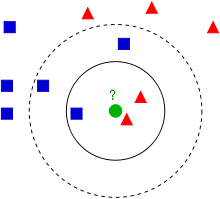
\includegraphics[]{220px-KnnClassification.png}
    \caption{An example of the KNN algorithm for classification.
    There are 2 classes in this example: Blue squares and Red triangles.
    The green circle needs to be classified.
    If K is 3 (the solid line), then the green circle will be classified as a red triangle.
    However, if K is 5 (the dotted line), then the green circle will be classified as a blue square.}
    \label{fig:knn}
\end{figure}


\subsubsection{Multi-Layer Perceptron}
%Talk about MLP Classifier here!!!
% Include MLP picture here I guess
The Multi-Layer Perceptron is a model that fits a function iteratively through a process called back-propagation.
The MLP classifier is a neural network model that is based on the structure of the human brain.
It consists of many layers beginning with an input layer.
The middle layers are called the "hidden layers" and are each assigned a weight.
Back propagation is used during training to adjust the weights in the hidden layers.
These adjustments are made in order to reach a more accurate prediction.
There can be many hidden layers of different depths.
The neural network is a versatile model that benefits from more training data with less risk of overfitting.
Training on very large datasets is known as Deep Learning.
% Probably need to say more about the MLP Classifier...
% Maybe some graphics and other bull jive. Maybe a algorithm???

\begin{figure}[htp]:
    \centering
    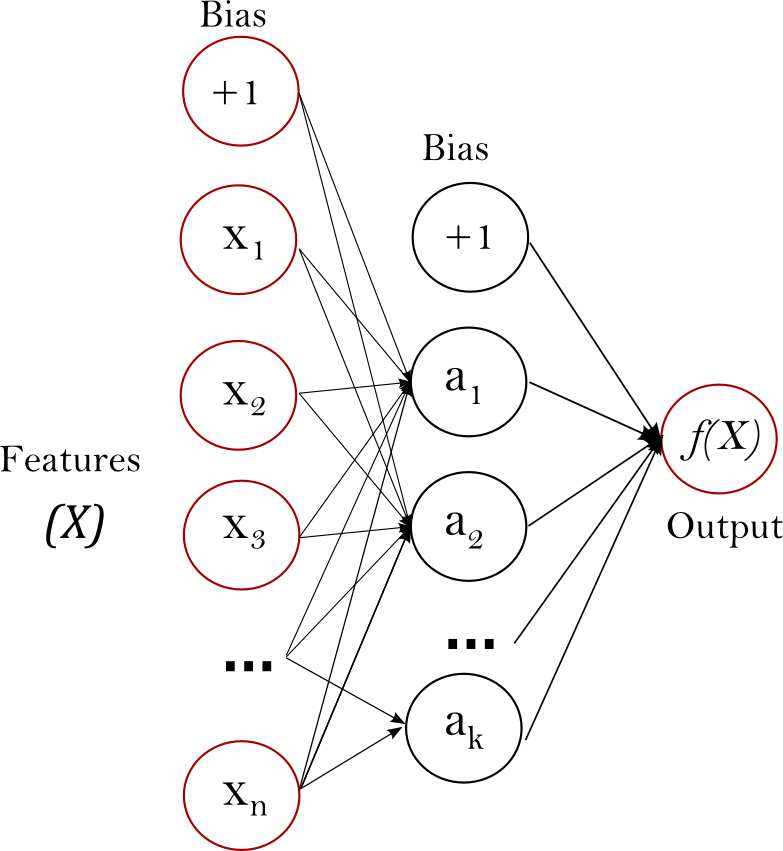
\includegraphics[scale=0.5]{multilayerperceptron_network.png}
    \caption{A Multi-Layer Perceptron.
    The middle or hidden layers are assigned weights that affect the selected class in classification.
    This model effectively models a function.}
    \label{}
\end{figure}

%include more here about MLP


\subsubsection{Naive Bayes}
%Talk about Naive Bayes classifier here!!
The Naive Bayes classifier is based on applying the Naive Bayes theorem \cite{zhang2004optimality}.
The naive assumption of Naive Bayes is the conditional independence between pairs of features given the label.
Bayes theorem states the following relationship:

\begin{equation}
    \label{eq:bayes}
    P(\theta|\textbf{D}) = P(\theta) \frac{P(\textbf{D} |\theta)}{P(\textbf{D})}
\end{equation}

In equation \ref{eq:bayes}, $\theta$ and \textbf{D} are events. 
P($\theta$|\textbf{D}) represents the probability of $\theta$ occurring given event \textbf{D} is true, where P(\textbf{D}) is the probability of observing event \textbf{D} alone.
Bayes Theorem will produce a probability of an event happening given another event using prior probabilities.
For example, say you wanted to predict the probability of both a stock falling and the DOW being down.
If you knew the probability of both falling independently you could use Bayes theorem to calculate the probability of both happening together.

Naive Bayes classifiers use an assumption of conditional independence between every pair of features given the value of the class variable. 
These over-simplified assumptions do not negatively affect the classifiers.
In fact, Naive Bayes classifiers work well in many real-world situations because of the conditional assumptions\cite{zhang2004optimality}.
Famously, it has performed well for document classification and spam filtering. 

\subsubsection{Regression Models}
%Talk about Regression models used here...
Regression models are utilized for predicting continuous values.
Specifically, regression is used for approximating a function given a set of inputs to yield output.
Linear regression is the simplest type and is concerned with fitting a linear combination of all training features.
Polynomial regression fits a polynomial combination to the training figures.
This can fit a function up to order N with the cost of complexity.

\begin{figure}[htp]
    \centering
    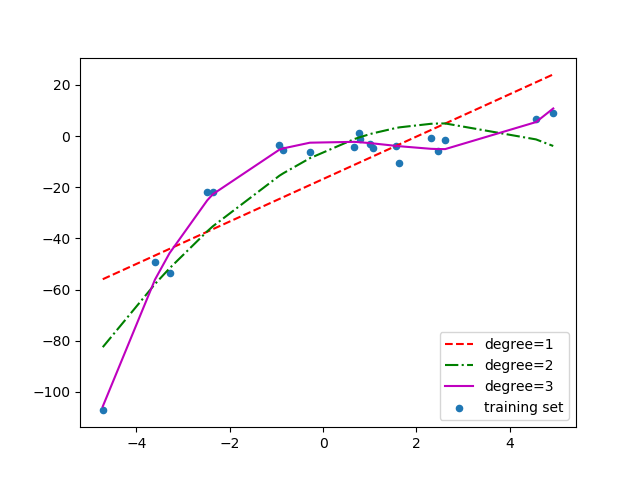
\includegraphics[width=\textwidth]{polynomialvslinearregression.png}
    \caption{3 example regression models fit to a set of points.
    A linear regression (red line) does not fit the data well.
    As the order rises the line will better fit the data.
    These higher order polynomial regression lines come at the cost of complexity and increasing the variance of the function.}
    \label{fig:repressionexample}
\end{figure}

% Put linear regression equation right here for the world to see YO

This project utilizes three regression models from Python's sci kit library.
The Naive Bayes\cite{sklearn_api}, logistic regression\cite{sklearn_api}, and svm regression\cite{sklearn_api} models are utilized for regression.

\subsection{Global Bathymetry Data}
The oceans of the Earth are humanities last frontiers.
Ironically, we knows very little about the bathymetry of these frontiers \cite{becker2009global}.
This is due to several factors including but not limited to: measurement techniques, sediment migration, tectonic activity, and the vast size of oceans.
This section is concerned with explaining the many measurement techniques for bathymetry and how they are used for creating global bathymetry grids.

\subsection{Echo Sounders (Multi Beam Echo Sounders)(Single Beam Echo Sounders) }

\begin{figure}[htp]
    \centering
    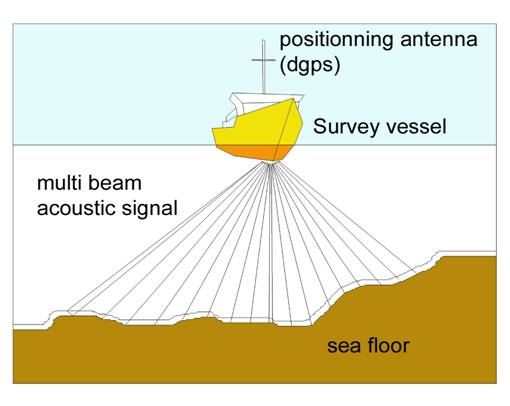
\includegraphics[width=\textwidth]{Geophy03-01.jpg}
    \caption{An \ac{MBES} system illustrated by a hull mounted sensor.
    The sensor ensonifies the sea floor and listens for the echo of the sound.
    The time the echo takes to return is used to measure the depth. 
    The illustration was taken from \cite{monacoWeb}.}
    \label{fig:MBES}
\end{figure}

Echo sounders have been mounted on vessels for decades to accurately measure bathymetry.
The purpose of this is often for a ship to avoid running aground.
This is where a ship strikes ground in a body of water.
Survey vessels have utilized \ac{MBES} systems to create reliable bathymetry charts \cite{farr1980multibeam}.
These charts give an accurate measurement of bathymetry in all water depths.
The downside of this method is the cost and time required to map global coverage.
A vessel must transport these sensors, and potentially require decades of expensive surveys to gain full global coverage.

\begin{figure}[htp]
    \centering
    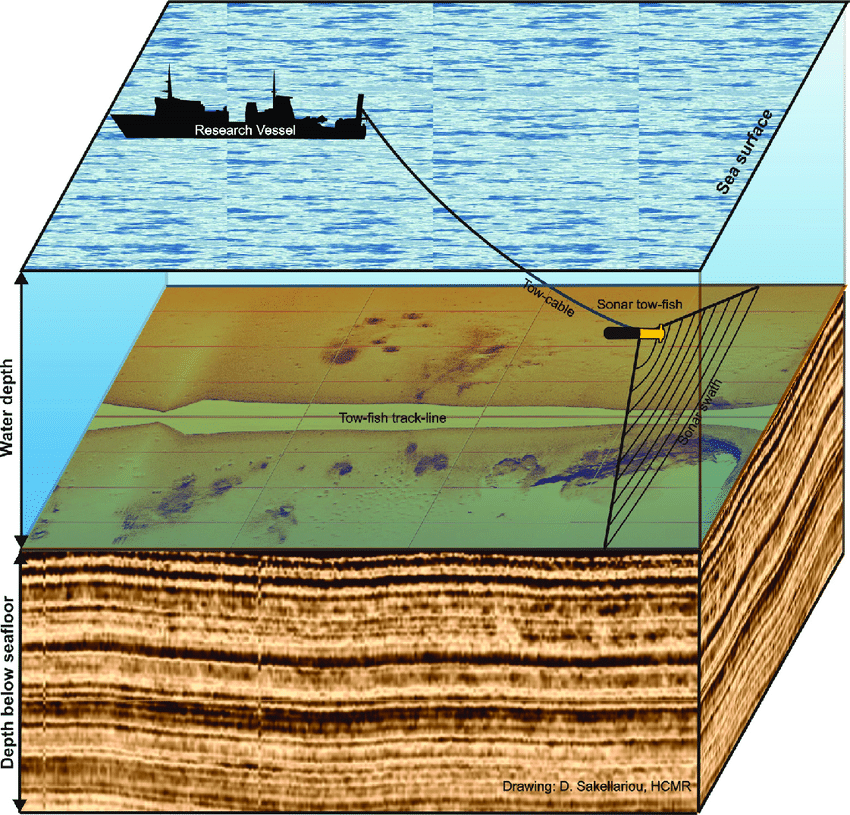
\includegraphics[width=\textwidth]{Schematic-presentation-of-the-side-scan-sonar-and-sub-bottom-profiling-survey-conducted.png}
    \caption{Sidescan sensor used by a survey ship via a tow fish.
    SideScan sonar is a type of \ac{SBES}.
    A tow fish is a sensor enclosing that is attached to a tow line from the stern of the vessel.
    This image was taken from \cite{sakellariou2015preliminary}.}
    \label{fig:sidescandemo}
\end{figure}


There are two main categories of echo sounders: \ac{MBES} and \ac{SBES}.
\ac{MBES} are large swath sonar based sensors.
They produce several artifacts including: bathymetry, backscatter, and salinity.
These sensors are used for a wide array of commercial and research applications.
See Figure~\ref{fig:MBES} for a illustration of \ac{MBES}.
Side-Scan sonar is a focused sonar system.
They produce "imagery" artifacts and will sense a smaller swath of ocean than \ac{MBES} sensors.
Side-Scan sonar is ideal for detecting objects on the ocean floor due to the image quality of the artifacts.
In general, SideScan systems are only used for object detection.
Figure \ref{fig:sidescandemo} shows an illustration of a towed SideScan sensor body.




%VERY VERY VERY IMPORTANT SECTION....2018 paper contains good content for my thesis!
\subsection{Satellite Derived Bathymetry (SDB)}
\ac{SDB} is a precise method of predicting coastal bathymetry. 
This method relies on the phenomena of light passing through a water column at a certain depth described by the Beer-Lambert law \cite{chybicki2018three}\cite{vinayaraj2016satellite}.
Sunlight passes through the water column and is reflected by the sediment at the bottom.
Satellites measure the attenuated light that is reflected from the bottom and uses the wavelength to estimate the depth of the column.
The technique accounts for atmospheric light absorption, water surface reflection, attenuation through and out of the column, and reflectance from the bottom sediment.
Clear waters are the best environment for this method, which has the potential to predict bathymetry with a small RMSE \cite{chybicki2018three}.

% Define RMSE in the machine learning lit review section for metrics!

\par
This method is important for its ability to predict swaths of bathymetry in shallow water where larger vessels can not sail.
Large swaths of shallow coastal waters are measured by \ac{SDB} in a cost and time-effective process.
An example where \ac{SDB} is useful is the marshlands of Louisiana where water depth is only deep enough for flat-bed vessels.
This method also has been used in the scope of national defense for predicting or identifying changes in shallow water bathymetry.
These changes can be caused by sediments or man-made objects. 

%Complex interaction between water column!!
\begin{figure}[htp]
    \centering
    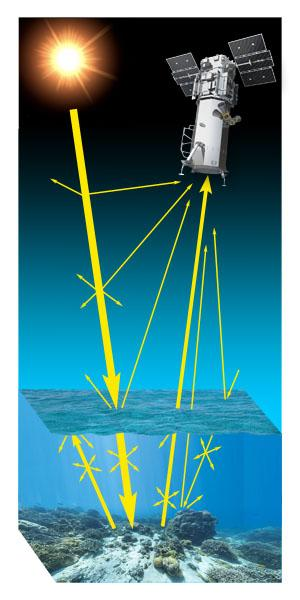
\includegraphics[scale=0.5]{CBYK292WkAAIkzH.jpg}
    \caption{\ac{SDB}.
    Sunlight penetrates the water column and reflects back into space where it is captured by a satellite.}
    \label{fig:sdb}
\end{figure}

\par
The limitations of the \ac{SDB} method are based on water depth and clarity.
%Reword this sentence!
As depth increases, light is unable to pass through the water column to the bottom.
The depth that light can penetrate is determined by the characteristics of the water.
Clear water will allow for much deeper depths to be predicted, whereas murky, cluttered water limits the maximum depth.
Environmental characteristics such as sediment composition and weather affect the clarity of water \cite{vinayaraj2016satellite}.

\par
Current \ac{SDB} models can predict bathymetry with a \ac{RMSE} of less than 2.5 meters at a maximum depth of 50 meters.
Work performed by~\cite{vinayaraj2016satellite} has improved the depth by using blue light-sensing techniques.
Work performed by~\cite{chybicki2018three} improved the accuracy by using advanced regression models when measuring the wavelengths.
\ac{SDB} models are ideal for coastal areas with high water visibility.

\subsection{Aggregated Earth Gravitational Models (EGM)}
Work performed by Smith and Sandwell~\cite{smith1994bathymetric,smith1997global} pioneered the use of Earth Gravitational Models (EGM) for predicting bathymetry.
They proposed that the relationship between seafloor topography and sea surface gravity is conveniently related~\cite{smith1994bathymetric}.
Their work identified the wavelength bands at which this relation holds true.
They identified the areas that could be predicted with this relationship and used sparse ship soundings to fill in the gaps of their predictions.
Areas with large seamounts found the correlation to be strongest, while areas of flat sediments found the correlation to be weakest.
They named this technique the "Inverse Nettleton Procedure" and used a simple linear regression model to exploit this correlation and improve existing aggregated datasets.

\begin{equation}
    b(x) = D(x) + s(x)g(x) \label{eq:egm}
\end{equation}

\par
Equation~\ref{eq:egm} represents the model created by~\cite{smith1994bathymetric}, where b represents the predicted bathymetry.
D represents a function of regional estimated depth via satellite.
s representing a regional scaling factor based on known sediments.
Finally, g represents inferred gravity from satellite imaging.

\par
Smith and Sandwell aggregated their predicted values from their \ac{EGM} with ship based \ac{MBES} Sounding sonar data.
The sonar data is sparse, but provides accurate readings of the ocean's bathymetry.
This aggregation yielded global coverage up to 81 degrees latitude.
The aggregation yielded prediction accuracy within ~100 meters in coastal waters and ~200 meters in the global ocean space.

%Discuss the STRM Global Dataset here in detail....
\par 
This work was later improved in~\cite{becker2009global}.
The model was substantially improved by increasing the number of ship soundings and increasing the aggregation sources.
Ten external datasets were aggregated for the SRTM30 grid.
Agencies in these sources include \ac{NAVO}, \ac{GEBCO}, \ac{NOAA}, \ac{NGA}, and \ac{JAMSTEC}.
These datasets include high-resolution coastal bathymetry from around the world and greatly increased the global accuracy.

%Spelling check big time bruh
\par
The limitations of aggregated \ac{EGM}s are based on "correlation uncertainty" and unknown ocean features.
Sediment density drives the correlation between sea surface gravity and bathymetry.
A dense geoid will generate greater sea surface gravity than a less dense geoid.
Flat sea floors with a less dense composition can appear lower than normal.
This is all controlled by the scaling factor described in~\cite{smith1994bathymetric} and shown in equation~\ref{eq:egm}.
However, there is not an optimal scaling factor for the entire world.
Identifying an optimal scaling factor for an area will require knowledge of the sediment type in the global scale.


\subsection{Machine Learning Optimized \ac{EGM}}\label{subsec:machine-learning-optimizedac}
The aggregated \ac{EGM} is a physics-based model that wants the relationship between gravity and bathymetry to be directly correlated.
This correlation is often non-trivial to define due to environmental factors.
The nondeterministic behavior is compensated by the scaling factor mentioned in the previous section.
Attempts to optimize this scaling factor have been made, and \ac{ML} has shown much promise in this regard.

\par
The work performed by~\cite{jena2012prediction} used \ac{ML} to optimize their gravitational regression models.
Instead of identifying an optimal scaling factor deterministically, they used an \ac{ANN} to optimize the scaling factor.
This was done using precise \ac{MBES} data as truth data and satellite altimeter data.
This method was tested on a localized swath of ocean in the Arabian Sea.

\par
This optimization improved upon the current physics models.
Their model could predict bathymetry within an \ac{RMSE} of ~129 meters for a section of flat sea-floor.
Geoids resulted in an \ac{RMSE} of ~179 meters.
Both of these results are globally similar to aggregated models, while boasting increased accuracy in their localized training area of the Arabian Sea.

%\subsection{Machine Learning Models}